% !TeX program = lualatex
% !TeX root = ./cv.tex
%%%%%%%%%%%%%%%%%%%%%%%%%%%%%%%%%%%%%%%
% Wenneker Resume/CV
% LaTeX Template
% Version 1.0 (3/5/2016)
%
% This template has been downloaded from:
% http://www.LaTeXTemplates.com
%
% Original author:
% Frits Wenneker (http://www.howtotex.com) with extensive modifications by 
% Vel (vel@LaTeXTemplates.com)
%
% License:
% CC BY-NC-SA 3.0 (http://creativecommons.org/licenses/by-nc-sa/3.0/
%
%%%%%%%%%%%%%%%%%%%%%%%%%%%%%%%%%%%%%%

%----------------------------------------------------------------------------------------
%	PACKAGES AND OTHER DOCUMENT CONFIGURATIONS
%----------------------------------------------------------------------------------------


\documentclass[a4paper,12pt]{memoir} % Font and paper size

%%%%%%%%%%%%%%%%%%%%%%%%%%%%%%%%%%%%%%%%%
% Wenneker Resume/CV
% Structure Specification File
% Version 1.0 (3/5/2016)
%
% This file has been downloaded from:
% http://www.LaTeXTemplates.com
%
% Original author:
% Frits Wenneker (http://www.howtotex.com) with extensive modifications by 
% Vel (vel@latextemplates.com)
%
% License:
% CC BY-NC-SA 3.0 (http://creativecommons.org/licenses/by-nc-sa/3.0/)
%
%%%%%%%%%%%%%%%%%%%%%%%%%%%%%%%%%%%%%%%%%

%----------------------------------------------------------------------------------------
%	PACKAGES AND OTHER DOCUMENT CONFIGURATIONS
%----------------------------------------------------------------------------------------

\usepackage{XCharter} % Use the Bitstream Charter font
% \usepackage[utf8]{inputenc} % Required for inputting international characters
% \usepackage[T1]{fontenc} % Output font encoding for international characters
\let\printglossary\relax
\usepackage{fontspec}
\usepackage{luatexja-fontspec}

\usepackage[top=1cm,left=1cm,right=1cm,bottom=1cm]{geometry} % Modify margins

\usepackage{graphicx} % Required for figures

\usepackage{flowfram} % Required for the multi-column layout

\usepackage{url} % URLs

\usepackage[usenames,dvipsnames]{xcolor} % Required for custom colours

\usepackage{tikz} % Required for the horizontal rule

\usepackage{enumitem} % Required for modifying lists

\usepackage{hyperref}
\usepackage{blindtext}
\usepackage{scrextend}
\setlist{noitemsep,nolistsep} % Remove spacing within and around lists

\setlength{\columnsep}{\baselineskip} % Set the spacing between columns

% Define the left frame (sidebar)
\newflowframe{0.2\textwidth}{\textheight}{0pt}{0pt}[left]
\newlength{\LeftMainSep}
\setlength{\LeftMainSep}{0.2\textwidth}
\addtolength{\LeftMainSep}{1\columnsep}
 
% Small static frame for the vertical line
\newstaticframe{1.5pt}{\textheight}{\LeftMainSep}{0pt}
 
% Content of the static frame with the vertical line
\begin{staticcontents}{1}
\hfill
\tikz{\draw[loosely dotted,color=RoyalBlue,line width=1.5pt,yshift=0](0,0) -- (0,\textheight);}
\hfill\mbox{}
\end{staticcontents}
 
% Define the right frame (main body)
\addtolength{\LeftMainSep}{1.5pt}
\addtolength{\LeftMainSep}{1\columnsep}
\newflowframe{0.7\textwidth}{\textheight}{\LeftMainSep}{0pt}[main01]

\pagestyle{empty} % Disable all page numbering

\setlength{\parindent}{0pt} % Stop paragraph indentation


\hypersetup{
  colorlinks=true,
  linkcolor=blue!50!red,
  urlcolor=blue!70!black
}

%----------------------------------------------------------------------------------------
%	NEW COMMANDS
%----------------------------------------------------------------------------------------

\newcommand{\userinformation}[1]{\renewcommand{\userinformation}{#1}} % Define a new command for the CV user's information that goes into the left column
\newcommand{\blankleft}[1]{\renewcommand{\blankleft}{#1}} % Define a new command for the CV user's information that goes into the left column
\newcommand{\cvheading}[1]{{\Huge\bfseries\color{RoyalBlue} #1} \\[-6pt]} % New command for the CV heading
\newcommand{\cvsubheading}[1]{{\Large\bfseries #1} \\} % New command for the CV subheading

\newcommand{\Sep}{\vspace{1em}} % New command for the spacing between headings
\newcommand{\SmallSep}{\vspace{0.5em}} % New command for the spacing within headings

\newcommand{\aboutme}[2]{ % New command for the about me section
\textbf{\color{RoyalBlue} #1}~~#2\Sep
}
	
\newcommand{\CVSection}[1]{ % New command for the headings within sections
{\Large\textbf{#1}}\par
\SmallSep % Used for spacing
}

\newcommand{\CVItem}[2]{ % New command for the item descriptions
\textbf{\color{RoyalBlue} #1}\\
#2
\SmallSep % Used for spacing
}

\newcommand{\bluebullet}{\textcolor{RoyalBlue}{$\circ$}~~} % New command for the blue bullets
 % Include the file specifying document layout and packages

%----------------------------------------------------------------------------------------
%	NAME AND CONTACT INFORMATION 
%----------------------------------------------------------------------------------------

\userinformation{ % Set the content that goes into the sidebar of each page
% Comment out this figure block if you don't want a photo
\begin{figure}
\hfill % Right align the photo
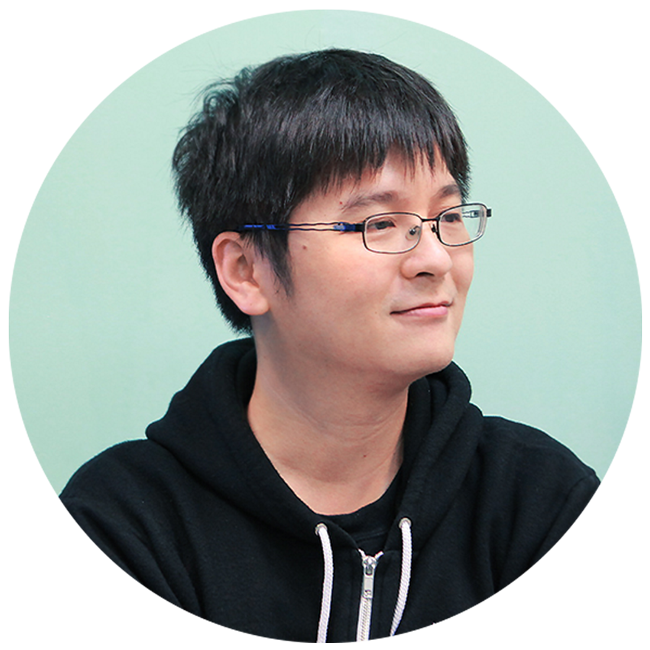
\includegraphics[width=0.6\columnwidth]{dorgon_photo_circle.png} % Your photo
\end{figure}

\begin{flushright}
\small % Smaller font size

張景照 \\ 
Ching Chao, Chang \\
Dorgon Chang \\


\Sep % Some whitespace

EMAIL: \\
%\textbf{dorgonman@}\\hotmail.com
%\url{dorgonman@hotmail.com} \\ % Your email address
\href{mailto:dorgonman@hotmail.com}{\textbf{dorgonman@}\\hotmail.com} \\


\Sep % Some whitespace

\textbf{BLOG:} \\ \href{http://dorgon.horizon-studio.net/}{dorgon.\\horizon-studio.net}

\Sep % Some whitespace
\Sep % Some whitespace


\textbf{GITHUB:} \\ \href{https://github.com/dorgonman}{github.com/\\dorgonman}

\vfill % Whitespace under this block to push it up under the photo
\end{flushright}
}


\blankleft{
% Comment out this figure block if you don't want a photo
  
  \begin{flushright}

  \end{flushright}
}
%----------------------------------------------------------------------------------------

\begin{document}

\userinformation % Print your information in the left column

\framebreak % End of the first column

%----------------------------------------------------------------------------------------
%	HEADING
%----------------------------------------------------------------------------------------

\cvheading{張景照(Dorgon Chang)} % Large heading - your name

\cvsubheading{Software Engineer} % Subheading - your occupation/specialization

%----------------------------------------------------------------------------------------
%	ABOUT ME
%----------------------------------------------------------------------------------------

\aboutme{About Me}{
  Professional game programmer with vast experince in game development 
  and DevOps automation.
  Currently working on Game Projects using UnrealEngine.
}

% 善長遊戲程式設計與流程自動化,擁有多個遊戲與VR專案開發經驗。
% 目前專注於研究UnrealEngine相關技術與應用。 game devlop techniques using UnrealEngine


\Sep % Some whitespace
%----------------------------------------------------------------------------------------
%	EXPERIENCE
%----------------------------------------------------------------------------------------

\CVSection{Experience}

%------------------------------------------------
\CVItem{2018-04-Current, \textit{NeoBards Entertainment}, Principal Programmer}{
  Working on Game Projects using UnrealEngine
  \begin{itemize}
    \item \href{https://www.youtube.com/watch?v=1uG2Y3MO4X0}{No Straight Roads} Optimization, Porting to Switch.
    \item Internal Projects using UnrealEngine: Architecture Design, OSS/OSSv2, AI, Quest, Dialogue, Optimization, and Localization workflow.
    \item \href{https://dwm.nexon.com/main}{Dynasty Warriors M}: CI/CD using Teamcity, AutomationTest flow for PGO/PSO gather, PatchSystem, and many other iOS/Android SDK required by game.
  \end{itemize}
}

\CVItem{2016/12-2018-03, \href{https://www.mai.ai/}{\textit{Medical Augmented Intelligence}}, Software Architect}{
  As a main programmer, develop following VR Projects using UnrealEngine:
  \begin{itemize}
    \item Acupuncture Simulation VR Project (B2B, Support Vive and Oculus)
    \item Body VR for Beginners {google store, Daydream}
    \item Medical Anatomy Training VR Project with Networking and Multiplayer (B2B, Support Vive and Oculus)
    \item CI/CD using AzureDevops
  \end{itemize}
}


\newpage

\blankleft % Print your information in the left column

\framebreak % End of the first column

\CVItem{2015/10-2016/11 , \textit{Gumi Taiwan}, Tech Lead}{
  As a Engineer Team Leader, 
  mentoring and sharing coding Skills with team members, 
  and make sure features are shipped in timely manner.
}

\CVItem{2013/10-2015/10 , \textit{Gumi Taiwan}, Software Engineer}{
  As a Game Client Programmer, 
  implement several funtions for 
  \begin{itemize}
    \item \href{https://www.youtube.com/watch?v=p3y6nao3rCU}{LINE Three Kingdoms Brave} using cocos2dx:
    \begin{itemize}
      \item Architecture Design and Implement
      \item Dialogue System
      \item Patch System
      \item CI/CD using jenkins
      \item Implement Database ORM with SOCI for client
      \item Boost Library Integration for Android and iOS
      \item Other Game Logics Implementation
    \end{itemize} 

    \item \href{https://www.youtube.com/watch?v=eYth6HNL5Go}{Crystal of Reunion}: 
    Establish Localization Workflow using Unity I2 Localization Plugin.
  \end{itemize} 
}



\CVItem{2012/11-2013/09 , \textit{Nubee Pte Ltd, Taiwan}, Software Engineer}{
  As a Game Client Programmer, 
  implement several funtions for 
  \begin{itemize}
    \item Fanta Swords
    \begin{itemize}
      \item CI/CD using Jenkins
      \item Patch System
      \item Texture Pack and Compress for Android(ETC1) and iOS(PVR)
    \end{itemize}
  \end{itemize}
}

\CVItem{2012/08-2012/11 , \textit{Nubee Pte Ltd, Singapore}, Software Engineer}{
  As a Game Client Programmer, 
  implement several funtions for 
  \begin{itemize}
    \item \href{https://www.youtube.com/watch?v=B0Ak4wmmKAA}{Samurai Empire}
    \begin{itemize}
      \item Porting in House C++ Game Engine to Android Platform.
      \item Social Network Binding for Facebook, twitter, renren, weibo and mixi
      \item Android GCM Notification
      \item Device Binding and Transfer
    \end{itemize}
  \end{itemize}
}

\CVItem{2011/08-2012/07 , \textit{Mandatory military service}}{

}
%------------------------------------------------

\newpage

\userinformation % Print your information in the left column

\framebreak % End of the first column
%----------------------------------------------------------------------------------------
%	EDUCATION
%----------------------------------------------------------------------------------------

\CVSection{Education}

%------------------------------------------------

\CVItem{2009/09-2011/06, 
National Chiao Tung University, 
Hsinchu, Taiwan,College of Computer Science, 
Institutes of Multimedia Engineering}
{
  Master of Science in Multimedia Engineering \\
  Master Thesis:\href{https://www.dropbox.com/s/w9d11qd79i5y4pl/master_thesis_dorgon_chang.pdf?dl=0} 
  {Measuring Difficulty and Complexity of Puzzle Games} \\
  Code Used in Thesis:\href{https://github.com/dorgonman/Cross_Block}
  {https://github.com/dorgonman/Cross\_Block}

}

\CVItem{2010/10-2011/04, 
University of Tokyo, Japan,
Department of Electrical Engineering and Information Systems
}{Exchange Student}

\CVItem{2005/09-2009/06, 
National Yunlin University of Science and Technology, Taiwan,
Information  Management}{Bachelor of Business Administration}
%------------------------------------------------


\Sep % Extra whitespace after the end of a major section
\Sep % Extra whitespace after the end of a major section
\Sep % Extra whitespace after the end of a major section
% \newpage


% \userinformation % Print your information in the left column

% \framebreak % End of the first column


%----------------------------------------------------------------------------------------
%	SKILLS
%----------------------------------------------------------------------------------------

\CVSection{Software Development Skills}


%------------------------------------------------

\CVItem{Knowledge}
{\begin{tabular}{p{0.3\textwidth} p{0.3\textwidth}}
 \bluebullet CI/CD & \bluebullet Networking \\
 \bluebullet Computer Graphics & \bluebullet Game AI \\
 \bluebullet iOS/Android Development & \bluebullet Cross Compiling \\
\end{tabular}}

%------------------------------------------------


%------------------------------------------------

\CVItem{Programming}
{\begin{tabular}{p{0.2\textwidth} p{0.2\textwidth} p{0.2\textwidth}}
\bluebullet C/C++ &  \bluebullet C Sharp & \bluebullet Java \\
\bluebullet Shell Script &  \bluebullet Python &  \bluebullet CMake \\
\end{tabular}}

%------------------------------------------------

\CVItem{Game Engine Experience}
{\begin{tabular}{p{0.2\textwidth} p{0.2\textwidth} p{0.2\textwidth}}
 \bluebullet Unreal Engine & \bluebullet cocos2d-x & \bluebullet Unity \\
 \bluebullet OGRE & \bluebullet UDK & \bluebullet HGE \\
\end{tabular}}

%------------------------------------------------



%------------------------------------------------

\CVItem{Project Management Software Experience}
{\begin{tabular}{p{0.2\textwidth} p{0.2\textwidth} p{0.2\textwidth}}
 \bluebullet Azure DevOps & \bluebullet Redmine & \bluebullet Trello \\
 \bluebullet Mantis & \bluebullet Jira\\
\end{tabular}}

%------------------------------------------------


%------------------------------------------------

\CVItem{Version Control}
{\begin{tabular}{p{0.2\textwidth} p{0.2\textwidth} p{0.2\textwidth}}
 \bluebullet GIT/GIT LFS & \bluebullet Perforce & \bluebullet SVN \\
\end{tabular}}

%------------------------------------------------

\newpage


\userinformation % Print your information in the left column

\framebreak % End of the first column

%----------------------------------------------------------------------------------------
%	Side Projects: UnrealEngine
%----------------------------------------------------------------------------------------

\CVSection{Side Projects: UnrealEngine}

%------------------------------------------------

{
  \begin{itemize}
    \item Horizon Dialogue Plugin, released on Aug 9, 2019: \\
        \href{https://www.unrealengine.com/marketplace/horizondialogue-plugin}
             {www.unrealengine.com/marketplace/horizondialogue-plugin} \\
    \item Horizon UI Plugin, released on Jun 27, 2016: \\
        \href{https://www.unrealengine.com/marketplace/horizon-ui-plugin}
             {www.unrealengine.com/marketplace/horizon-ui-plugin} \\
    \item Horizon Tween Plugin, released on Oct 20, 2016: \\
        \href{https://www.unrealengine.com/marketplace/horizontween-plugin}
             {www.unrealengine.com/marketplace/horizontween-plugin} \\
    \item Horizon Framework Plugin, released on Feb 24, 2018: \\
          \href{https://www.unrealengine.com/marketplace/horizonframework-plugin}
               {www.unrealengine.com/marketplace/horizonframework-plugin} \\
    \item Horizon Interact Plugin, released on Jan 4, 2021: \\
          \href{https://www.unrealengine.com/marketplace/en-US/product/horizon-interact-plugin}
              {https://www.unrealengine.com/marketplace/en-US/product/horizon-interact-plugin}  \\
    \item Horizon Quest Plugin, released on Aug 29, 2021: \\
              \href{https://www.unrealengine.com/marketplace/en-US/product/horizon-quest-general-purpose-quest-graph-system}
                  {https://www.unrealengine.com/marketplace/en-US/product/horizon-quest-general-purpose-quest-graph-system}  \\
              
    \item Contribute Bug fix Code to UnrealEngine version 
    \href{https://www.unrealengine.com/en-US/blog/unreal-engine-49-released}{4.9}, 
    \href{https://www.unrealengine.com/en-US/blog/unreal-engine-4-14-released}{4.14}, 
    \href{https://www.unrealengine.com/en-US/blog/unreal-engine-4-15-released}{4.15},  
    \href{https://www.unrealengine.com/en-US/blog/unreal-engine-4-19-released}{4.19}, 
    \href{https://www.unrealengine.com/en-US/blog/unreal-engine-4-21-released}{4.21}, 
    \href{https://www.unrealengine.com/en-US/blog/unreal-engine-4-22-released}{4.22}, 
    \href{https://docs.unrealengine.com/latest/INT/Support/Builds/ReleaseNotes/4_24/}{4.24}, 
    \href{https://docs.unrealengine.com/5.0/en-US/unreal-engine-5-0-release-notes/}{5.0},
    \href{https://docs.unrealengine.com/5.2/en-US/unreal-engine-5.2-release-notes/}{5.2},
    \href{https://docs.unrealengine.com/5.3/en-US/unreal-engine-5.3-release-notes/}{5.3},
    \href{https://docs.unrealengine.com/5.4/en-US/unreal-engine-5.4-release-notes/}{5.4}, you can find my name "dorgon chang" or "dorgonman" in contributors list. \\


    \item Contribute Bug fix Code to 
    \href{https://github.com/git/git/pull/977}{git-p4} 

  \end{itemize}

}
%------------------------------------------------

\Sep % Extra whitespace after the end of a major section
\Sep % Extra whitespace after the end of a major section
\Sep % Extra whitespace after the end of a major section


%----------------------------------------------------------------------------------------
%	Honors
%----------------------------------------------------------------------------------------

\CVSection{Honors}
\begin{itemize}
  \item The Phi Tau Phi Scholastic Honor Society (2009)
\end{itemize}


\Sep % Extra whitespace after the end of a major section
\Sep % Extra whitespace after the end of a major section
\Sep % Extra whitespace after the end of a major section
%----------------------------------------------------------------------------------------
%	Language
%----------------------------------------------------------------------------------------

\CVSection{Language Skills}
\begin{itemize}
  \item Mandarin Chinese: Native Speaker
  \item English: Business Level, New Toeic 805(CEF B2), 2016
  \item Japaness: Business Level, JLPT Level 1 339/400, 2006
\end{itemize}


\Sep % Extra whitespace after the end of a major section
\Sep % Extra whitespace after the end of a major section
\Sep % Extra whitespace after the end of a major section

\end{document}